\documentclass{article} % For LaTeX2e
\usepackage{nips15submit_e,times}
\usepackage{hyperref}
\usepackage{url}
\usepackage{amssymb}
\usepackage{booktabs}
\usepackage{enumitem}
\usepackage{amsmath}
\usepackage{graphicx}

%\documentstyle[nips14submit_09,times,art10]{article} % For LaTeX 2.09

\title{Accelerating Multimodal Sequence Retrieval with Convolutional Networks}


\author{
Colin Raffel\\
LabROSA\\
Columbia University\\
New York, NY 10027\\
\texttt{craffel@gmail.com}
\And
Daniel P.~W.~Ellis\\
LabROSA\\
Columbia University\\
New York, NY 10027\\
\texttt{dpwe@ee.columbia.edu}
}

\newcommand{\fix}{\marginpar{FIX}}
\newcommand{\new}{\marginpar{NEW}}

\nipsfinalcopy % Uncomment for camera-ready version

\begin{document}

\maketitle

\begin{abstract}
Given a large database of sequential data, a natural problem is to find the entry in the database which is most similar to a query sequence.
Warping-based similarity metrics such as the dynamic time warping (DTW) distance can be prohibitively expensive when the sequences are long and/or high-dimensional.
To mitigate these issues, \cite{raffel2015large} utilizes a convolutional network to map sequences of feature vectors to downsampled sequences of binary vectors.
On the task of matching synthetic renditions of pieces of music to a large database of audio recordings of songs, this approach was able to efficiently discard 99\% of the database with high confidence.
We extend this approach to the multimodal setting where rather than synthetic renditions, a matrix representation of the piece's score is used, demonstrating that this approach is adaptable to the changes in the underlying representation.
\end{abstract}

\section{Introduction}
\label{sec:intro}

The ability to compute a similarity metric for sequences of feature vectors is necessary for the task of retrieving the most similar entry (nearest-neighbor search) in a database of sequences.
A natural way to compare sequences is to first find their optimal alignment and then compute the total distance between aligned feature vectors.
Aligning the sequences before computing the total distance makes metrics of this type robust to timing distortions (e.g.\ offset, skew, or cropping), and can be achieved in quadratic time using dynamic programming \cite{rakthanmanon2012searching}.
For feature vectors which can be effectively compared with Euclidean distance (e.g.\ those with continuously-valued features), the most commonly used method of this type is dynamic time warping (DTW) \cite{sakoe1978dynamic}, which will be the focus of this work.

The quadratic cost of the dynamic programming-based alignment operation can make nearest-neighbor search infeasible for databases with many entries and/or long sequences.
Furthermore, traditional DTW involves computing the pairwise distance between all feature vectors in the two sequences being compared, which can outweigh the cost of alignment for high-dimensional data.
A common way to avoid these costs is to use ``pruning'' techniques, which use heuristics to skip a large portion of the database.
A wide variety of pruning methods have been proposed; \cite{rakthanmanon2012searching} gives an overview and shows that their successful application can enable nearest-neighbor search in databases with trillions of sequences.
Despite their benefits, pruning methods typically rely on various constraints on the comparisons being made, such as the query sequence always being a subsequence of its correct match in the database and that the total number of aligned frames is fixed.
Furthermore, these methods suffer losses in efficiency when sequences are oversampled and/or high dimensional.

An alternative approach is to compute fixed-length embeddings of sequences and use Euclidean distance in the embedded space as a proxy for sequence similarity.
For example, \cite{papapetrou2011embedding} computes an embedding as the DTW distance between each sequence and a small collection of ``reference'' sequences which are chosen to optimize retrieval quality.
The resulting embeddings can provide state-of-the-art pruning both in terms of accuracy and speed, but rely on the same assumptions discussed in the previous paragraph.
A different collection of embedding-based approaches are ``audio fingerprinting'' techniques \cite{wang2003industrial}, which seek to produce a single hash vector for a sequence which is invariant to noise and corruptions.
These approaches have proven to be extremely effective for exact retrieval, but are ineffective in settings where the desired match for a query sequence differs substantially in content.
As a result, ``soft fingerprinting'' methods have been proposed which are more flexible to differences in content \cite{van2015audio}, but their performance is meager compared to stricter fingerprinting methods.

To avoid these issues, in \cite{raffel2015large} we proposed a learning-based method which utilizes a convolutional network to map sequences of feature vectors to downsampled sequences of binary vectors.
The resulting ``hash sequences'' can be much more efficiently compared using dynamic time warping, which enables flexible, problem-adaptive pruning.
In this paper, we will show that this framework is additionally flexible to multimodal settings, where the sequences being compared represent different types of data.

\section{Learning a More Efficient Representation for DTW}

Because the constraints and requirements of a sequence retrieval problem can vary based on the data, a natural question is whether sequence comparison can be made more efficient in a learning-based manner.
In particular, if sequences are very long and high-dimensional, mapping sequences to shorter, lower-dimensional sequences such that similarity is preserved would provide quadratic speed gains when comparing sequences with DTW.
Motivated by this possibility, in \cite{raffel2015large} we developed a system with the following capabilities:
\begin{description}[topsep=1pt,itemsep=-1pt,leftmargin=10pt]
\item[Maps to a Hamming space:] By replacing continuous-valued feature vectors with bitvectors in an embedded Hamming space, computing the distance between a pair of feature vectors simplifies to a single exclusive-or and a table lookup: The exclusive-or of two bitvectors $a$ and $b$ will yield a bitvector consisting of $1$s where $a$ and $b$ differ and $0$s elsewhere, and the number of $1$s in all bitvectors of length $D$ can be precomputed and stored in a table of size $2^D$.
\item[Downsamples sequences:] Rather than creating a one-to-one correspondence between the original featured vectors and mapped bitvectors, groups of subsequent feature vectors are mapped to a single bitvector, giving a quadratic increase in efficiency.
\item[Preserves similarity:] The system is trained with an objective which seeks to produce a mapping where aligned feature vectors from matching sequences have a small Hamming distance in the embedded space, and non-matched feature vectors have a large distance.
\item[Learns its representation:] Our approach is entirely data-driven, which allows it to adapt to different problem settings including multimodal data, as we show in Section \ref{sec:multimodal}.
\end{description}

In this section, we will given an overview of our system; for a more thorough description, see \cite{raffel2015large} \S3.

\subsection{Similarity-Preserving Hashing}

To begin with, our model requires a training set of sequences which are both matched and aligned.
This training set can be constructed by obtaining a collection of sequences for which matching pairs are known, and then using DTW to find the optimal alignment of feature vectors in matching sequences.
We call this collection of matching feature vectors $\mathcal{P}$, such that $(x, y) \in \mathcal{P}$ indicates that $x$ is the feature vector in some sequence from one modality which has been aligned to $y$ in a matching sequence from another modality.
We then construct $\mathcal{N}$, a set of ``dissimilar'' pairs, by repeatedly randomly choosing two pairs $(x_1, y_1), (x_2, y_2) \in \mathcal{P}$ and swapping their entries to construct $(x_1, y_2), (x_2, y_1) \in \mathcal{N}$.
Given this training data, our goal is to map feature vectors to a Hamming space where pairs in $\mathcal{P}$ have a small distance and pairs in $\mathcal{N}$ have a large distance.
Motivated by the multimodal hashing technique of \cite{masci2014multimodal}, we use the following objective function to measure the quality of the mapping:
\begin{equation*}
\mathcal{L} = \frac{1}{|\mathcal{P}|} \sum_{(x, y) \in \mathcal{P}} \| f(x) - g(y) \|_2^2  - \frac{\alpha}{|\mathcal{N}|} \sum_{(a, b) \in \mathcal{N}} \max(0, m - \|f(a) - g(b) \|_2)^2
\end{equation*}
where $f$ and $g$ are learned nonlinear functions, $\alpha$ is a parameter to control the importance of separating dissimilar items, and $m$ is a target separation of dissimilar pairs.
As long as $f$ and $g$ are differentiable functions, this system can be optimized by using gradient descent to adjust the parameters of $f$ and $g$ such that $\mathcal{L}$ is minimized.

After minimizing $\mathcal{L}$ on a training set, pairs of sequences of feature vectors in either modality can then be mapped to pairs of sequences of hash vectors using $f$ and $g$.
Once mapped, we can perform DTW much more efficiently to compute a distance between the hash sequences.
Ideally, the DTW distance between the original sequences will be well-approximated by the DTW distance of the hash vectors, which can be computed more efficiently.
Overviews of DTW and its calculation can be found in \cite{muller2007dynamic, rakthanmanon2012searching} and \cite{raffel2015large} \S 2.2.

\subsection{MIDI to Audio Matching Experiment}
\label{sec:hashing}

We tested the effectiveness of this approach on the task of matching synthetically generated renditions of pieces of music to recordings of the same pieces in a large database of audio recordings.
For the first modality, synthetic recordings of music were obtained by using the \texttt{fluidsynth} program to synthesize musical scores in the form of MIDI files, a widely used format for transcribing music.
For the second, we used audio recordings from the Million Song Dataset (MSD) \cite{bertin2011million,schindler2012facilitating}.
The goal was therefore to efficiently match a synthetic rendition to its original recording among the million recordings in the MSD.
For both modalities, we used feature vectors of log-magnitude, constant-Q (i.e.\ log-frequency) spectra with 48 frequency bins from 130 to 1047 Hz.
To normalize differences in tempo, we estimated beat locations and computed spectrograms (sequences of spectra) on a timescale where each spectrum corresponded to the span of an estimated beat.
An example of this representation can be seen in Figure \ref{fig:sims_and_dtws}(a).
MIDI and audio analyses were performed with \texttt{pretty\char`_midi} \cite{raffel2014pretty_midi} and \texttt{librosa} \cite{mcfee2015librosa,mcfee2015librosa_scipy} respectively.

\begin{figure}
  \centering
  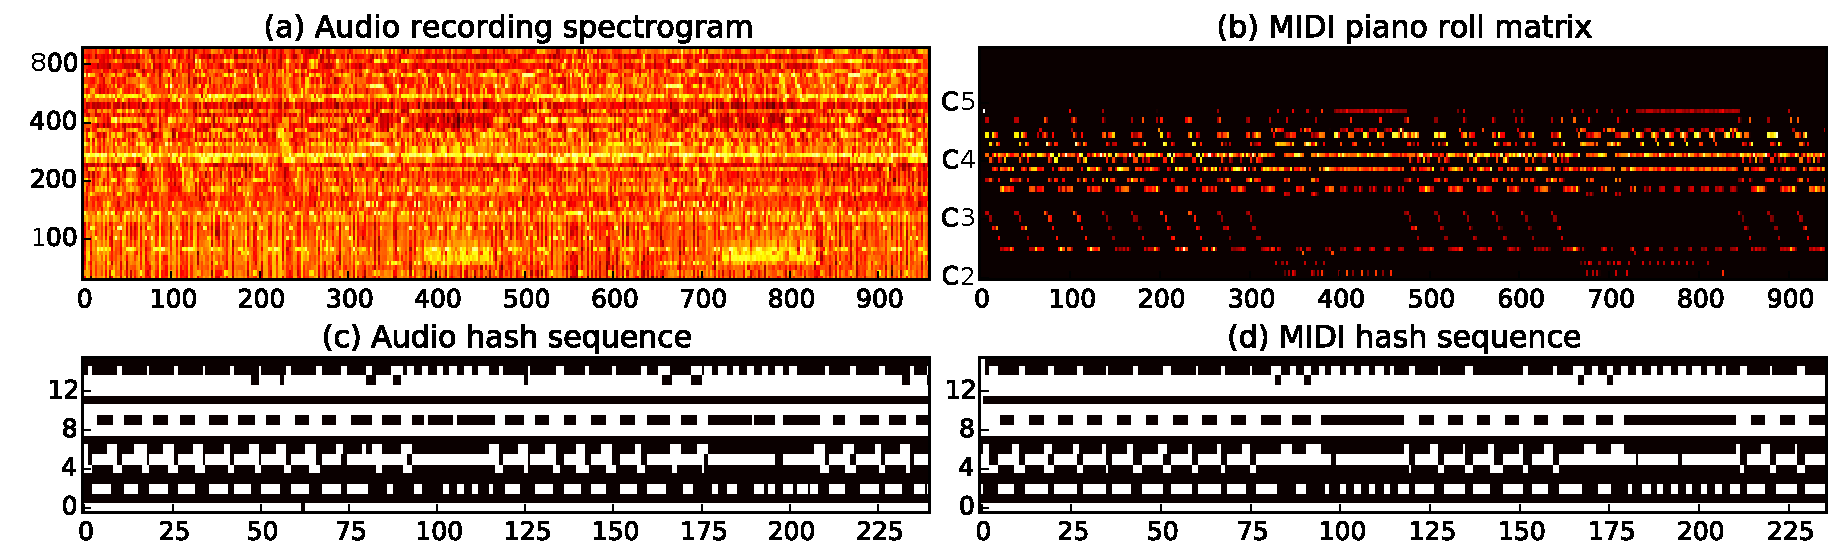
\includegraphics[width=\textwidth]{sims_and_dtws.pdf}
  \caption{Example audio spectrogram and MIDI piano roll and their corresponding hash sequences (cf.\ \cite{raffel2015large} Figure 2).
  (a) Normalized beat-synchronous constant-Q spectrogram of an audio recording, with frequency in Hz on the vertical axis and beat index on the horizontal axis.
  (b) Piano roll matrix for a transcription of the same song, with notes on the vertical axis and beat indices on the horizontal axis.
  (c) Resulting hash sequence for the audio spectrogram, with pooled beat indices and Hamming space dimension on the horizontal and vertical axes respectively.
  (d) Hash sequence for the MIDI piano roll.}
  \label{fig:sims_and_dtws}
\end{figure}

In \cite{masci2014multimodal}, dense feed-forward neural networks are used for the learnable functions $f$ and $g$; we instead opted for convolutional networks due to the fact that sequential data tends to exhibit invariances over time which convolutional networks can learn to model with fewer parameters.
In addition, by utilizing max-pooling layers to downsample over time, the resulting hash sequences can be made shorter, which makes computing the DTW distance quadratically faster.
In our experiments, we used the same network structure for $f$ and $g$.
Spectrograms were fed into a convolutional layer with sixteen $5 \times 12$ filters, followed by a $2\times2$ max-pooling layer, another convolutional layer with thirty two $3\times3$ filters, another $2\times2$ max-pooling layer, two dense layers with 2048 units, and a final dense output layer.
Each layer in the network used a rectified linear unit (ReLU) nonlinearity except the last, which as in \cite{masci2014multimodal} used a $\tanh$ nonlinearity.
This allows us to obtain binary hash vectors by testing whether each output dimension is greater or less than zero.
We used an output dimensionality of 16 so that the resulting hash vectors could be represented as 16-bit unsigned integers.
All weight matrices and filters were initialized using He et al.'s method \cite{he2015delving}, and all biases were initialized to zero.
Our model was implemented using \texttt{theano} \cite{bastien2012theano,bergstra2010theano} and \texttt{lasagne} \cite{dieleman2015lasagne}.

For training data, we assembled a collection of MIDI files which were determined to be high-quality transcriptions of corresponding audio recordings.
We held out 10\% of this training set as a validation set, which was used to estimate the performance of our networks for early stopping and hyperparameter tuning, described below.
We normalized all input feature vectors by their $L^2$-norm, then z-scored (standardized) feature vectors according to the statistics of the training set.
Training data was presented to the network as minibatches of 50 randomly-cropped length-100 subsequences.
To train the networks, we backpropagated the gradient of $\mathcal{L}$ through the networks' parameters and used RMSProp for optimization \cite{tieleman2012lecture}.
After each 100 minibatches, we tested whether the loss $\mathcal{L}$ computed on the validation set was was less than $99\%$ of the previous lowest; if it was, we trained for 1000 more iterations (minibatches).

To maximize performance, we performed Gaussian Process-based hyperparameter optimization using Whetlab, which was a web API implementing the techniques described in \cite{snoek2012practical}.
The scale of the validation loss will vary with the $\alpha$ and $m$ regularization hyperparameters, so as an objective we instead used the Bhattacharyya coefficient between the distributions of distances between hash vectors produced from matching and non-matching sequences from the validation set.
A small Bhattacharyya coefficient therefore indicates that a given system produces hash vectors which preserve similarity.
We used Whetlab to optimize the number of convolutional/pooling layers, the number and size of the fully-connected layers, the RMSProp learning rate and decay parameters, and the $\alpha$ and $m$ regularization parameters of $\mathcal{L}$.
The best performing hyperparameter configuration produced a Bhattacharyya coefficient of $0.488$, indicating a high degree of separation between the distributions.

After training a model which effectively maps sequences of feature vectors to shorter sequences of binary vectors, we evaluated its performance on a held-out test set of MIDI files for which we knew a priori the correct match in the MSD.
For each MIDI file in our test set, we computed its hash sequence representation and the resulting DTW distance to every hash sequence of every audio recording in the MSD.
To measure performance, we then ranked MSD entries according to their hash sequence DTW distance and determined the rank of the correct match.
In our test set of 1,537 pairs, our system achieved a mean reciprocal rank of $0.241$, indicating that the correct match tended to be ranked highly.
To further measure performance, we report the percentage of MIDI files in the test set where the correct match in the MSD ranked below a certain threshold for various thresholds in Table \ref{tab:rank-percentages}(a).

As can be seen from this table, the correct entry in the MSD only had the smallest distance about 15.2\% of the time, which suggests that this approach cannot reliably used in isolation.
However, because it was able to rank the correct entry in the top 1\% of the MSD (corresponding to 10,000 entries) 95.9\% of the time, it can instead be used as an effective pruning method.
Our best-performing model included two 2$\times$2 max-pooling layers, which resulted in the number of hash vectors in a given sequence being 1/4 the number in the corresponding feature vector sequence.
This, combined with the speed-up obtained by using binary vectors instead of continuously-valued ones, resulted in our approach being about 100 times faster than standard DTW on the raw feature vectors.
As a result, a concise way to state the success of our system is that it is able to discard 99\% of entries of the MSD in 1\% of the time.

\begin{table}
  \begin{center}
    \begin{tabular}{l l l l l l l l l l l l}
      \toprule
      & \multicolumn{5}{c}{(a) Synthesized MIDI} & &  \multicolumn{5}{c}{(b) Piano roll} \\
      \cmidrule{2-6}
      \cmidrule{8-12}
      \textbf{Rank} & 1 & 10 & 100 & 1000 & 10000 & & 1 & 10 & 100 & 1000 & 10000 \\
      \textbf{Percent $\le$} & 15.2 & 41.6 & 62.8 & 82.7 & 95.9 & & 10.9 & 34.6 & 55.6 & 74.9 & 92.8 \\
      \bottomrule
    \end{tabular}
  \end{center}
  \caption{Percentage of MIDI/MSD pairs where the DTW distance ranked below each threshold, using (a) the synthesized MIDI spectrogram or (b) the MIDI piano roll as a representation.}
  \label{tab:rank-percentages}
\end{table}

\section{Shared Representations for Multimodal Sequences}
\label{sec:multimodal}

Our proposed system is structured to learn mappings from two different modalities thanks to the fact that two separate networks $f$ and $g$ are trained.
Despite this capability, in \cite{raffel2015large} we utilized a representation of MIDI files which is similar to the one used for audio recordings.
One drawback of using the constant-Q spectra of the synthesized MIDI files as feature vectors is that the resulting feature extraction pipeline is inefficient; for a complex MIDI file it can take tens of seconds.
In addition, utilizing this representation does not test the multimodal capabilities of our model.

We therefore repeated the experiment from \cite{raffel2015large} using a representation of MIDI data which is much more efficient to calculate and substantially different than the one used for audio files.
Instead of synthesizing the MIDI file and computing a constant-Q spectrogram, we instead computed a beat-synchronous ``piano roll'' matrix directly from the MIDI data itself.
A piano roll matrix $P$ is constructed such that $P[i, j] > 0$ denotes that note $i$ is playing on some instrument during the $j$th beat, and $P[i, j]$ is $0$ otherwise.
An example piano roll matrix can be seen in Figure \ref{fig:sims_and_dtws}(b).
Raw MIDI data can be readily converted to this format; for complex MIDI files, constructing such a matrix takes tens of milliseconds using \texttt{pretty\char`_midi}'s \texttt{get\char`_piano\char`_roll} and \texttt{get\char`_beats} functions \cite{raffel2014pretty_midi}.
While the resulting representation is still a time-frequency matrix, it contains substantially less information (e.g.\ notes played on different instruments have the same representation) and is not directly comparable to the spectrograms we used for audio files.

For ease of comparison, we utilized the exact same system as outlined in Section \ref{sec:hashing} except that we replaced the spectrograms of synthesized renditions with beat-synchronous piano roll matrices.
After training on this representation, the hashing network achieved a Bhattacharyya coefficient of $0.538$ which indicates that the networks succesfully preserved similarity, although not as effectively as when spectrograms of synthesized MIDI files were used as a feature representation.
The resulting hash sequences for the audio spectrogram shown in Figure \ref{fig:sims_and_dtws}(a) and the MIDI piano roll shown in \ref{fig:sims_and_dtws}(b) can be seen in Figure \ref{fig:sims_and_dtws}(c) and \ref{fig:sims_and_dtws}(d) respectively, which at a high level appear much more similar than the original feature vector sequences.

When evaluated on the task of matching our test set of MIDI files to the MSD, the model trained on piano roll matrices performed slightly worse than the system outlined in Section \ref{sec:hashing}, as can be seen in Table \ref{tab:rank-percentages}(b).
In particular, only 92.8\% (vs. 95.9\%) of the correct MSD matches for the MIDI files in the test set ranked below 10,000 (1\% of the MSD).
While this difference is significant, it nevertheless demonstrates that our system was able to learn an effective mapping despite the fact that the feature representations in each modality were substantially different.

\section{Future Work}

In this paper, we have summarized the system proposed in \cite{raffel2015large} for mapping sequences of feature vectors to shorter sequences of hash vectors, and have shown that it is robust to multimodal problem settings.
Given the success of this approach on the MIDI-to-audio recording matching experiment described in Section \ref{sec:hashing}, we are interested in applying it to other large-scale cross-modality sequence retrieval tasks.
One source of difficulty with using our system is that it requires a training set of matched and aligned sequences.
We are currently investigating methods to relax this constraint by embedding sequences of feature vectors as fixed-length vectors in a common space where similarity is preserved.
This approach will also replace the DTW-based comparison of hash sequences with a simple distance calculation, which could afford further efficiency gains.
We are also interested in experimenting with larger Hamming space dimensionalities, which may increase accuracy at the cost of a higher memory requirement for the pre-computed binary vector distance table.
For researchers interested in verifying and extending our results, all of the code used in these experiments is available online.\footnote{\href{https://github.com/craffel/midi-dataset}{\texttt{https://github.com/craffel/midi-dataset}}}

\bibliographystyle{unsrt}
\small
\bibliography{refs}

\end{document}
